\section{Abstract model for DAE units}

It is better to draw easier-to-understand pictures. Explanation: \ldots Call those DNA sequences ``glues''. Binding, tile and glue complexity. Note those twice longer sticky ends on the bottom line.

In following examples this model will be set up to act similarly like $\NP$: $\exists y \; R(x,y)$. Although existence is not sure, it is very likely. Predicate $R$ will be ``enumerable in polynomial time'' for $x \in L$. In this context, {\em enumerable in polynomial time} will mean number of bindings, not number of biosteps. This can be assumed due to Turing universality of this model in $O(1)$ biosteps -- biostep complexity is not restrictive\footnote{From Turing's thesis, Turing machine is the most universal model.} and will be required to be $O(1)$ due to its lab complexity. On the other hand the binding complexity will be very important, we will be interested even in constants. This is because the less binding complexity, the less probability of error.

Note that the word on the bottom line can be restricted to belong to arbitrary regular language.

%!% odhady se dají zmenšit pomocí #E místo #V^2
%!% spodní řádek má 2x tak dlouhý lepidla !! vysvětlit proč

\begin{figure}[h]
\begin{center}
	\begin{subfigure}[b]{0.31\textwidth}
		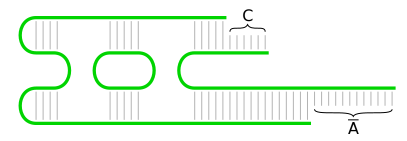
\includegraphics[width=\textwidth]{./figures/tile_model/DNA_struct.pdf} % 115mm
		\caption{Corner DAE unit}
		\label{fig:DNA_struct}
	\end{subfigure}
	\begin{subfigure}[b]{0.472\textwidth}
		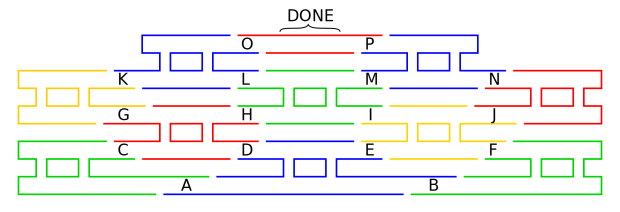
\includegraphics[width=\textwidth]{./figures/tile_model/DNA_assembly.pdf} % 175mm
		\caption{Scheme of self-assembly}
		\label{fig:DNA_assembly}
	\end{subfigure}
	\begin{subfigure}[b]{0.190\textwidth}
		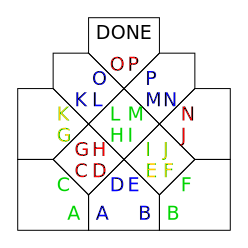
\includegraphics[width=\textwidth]{./figures/tile_model/abstract_model.pdf} % 70mm
		\caption{Abstract model}
		\label{fig:abstract_model}
	\end{subfigure}
	\caption{Evolution of abstract model from DAE units to tiles.}
	\label{fig:evolution}
\end{center}
\end{figure}
